% https://tex.stackexchange.com/questions/7814/nested-tikz-nodes

\documentclass{minimal}

\usepackage{tikz}
\usetikzlibrary{positioning,fit,calc}
\begin{document}

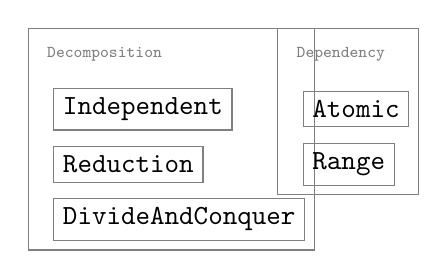
\begin{tikzpicture}[
  node distance=7mm,
  title/.style={font=\fontsize{6}{6}\color{black!50}\ttfamily},
  typetag/.style={rectangle, draw=black!50, font=\ttfamily, anchor=west}
]
  \node (decomp) [title] { Decomposition };

  \node (di) [below=of decomp.west, typetag, xshift=2mm] { Independent };
  \node (dr) [below=of di.west, typetag] { Reduction };
  \node (dnc) [below=of dr.west, typetag] { DivideAndConquer };

  \node [draw=black!50, fit={(decomp) (di) (dr) (dnc)}] {};

  \node (dep) at (3cm, 0) [title] { Dependency };

  \node (da) [below=of dep.west, typetag, xshift=2mm] { Atomic };
  \node (dr) [below=of da.west, typetag] { Range };

  \node [draw=black!50, fit={(dep) (dr) (da)}] {};
\end{tikzpicture}
\end{document}